\documentclass[10pt]{beamer}
\usepackage{pgf}
\usepackage{booktabs}
\usepackage{array}
\usepackage{ragged2e}
% \usepackage{booktabs}
%Information to be included in the title page:
\title{Elite individuals, insitutions, and economic growth accounting}
\author{James Xu}
\institute{ECON 442, Duke University}
\date{April 11, 2024}
\usefonttheme[onlymath]{serif}

\begin{document}
\setbeamertemplate{navigation symbols}{}

\frame{\titlepage}

\begin{frame}{Table of Contents}
    \tableofcontents
\end{frame}
\section{Intro}
\begin{frame}
    \frametitle{Research Question}
    \begin{block}{What is the relationship between elite students, academic institutions, and economic growth?}
        \begin{itemize}
            \item Are there outsized returns to economic growth when there are more academic elites?
        \end{itemize}
    \end{block}
    \begin{exampleblock}{Method}
        Through this paper, I investigate the relationship between the number of top-ranked universities, share of top math students,
        IMO scores, and GDP per capita growth to analyze these questions.
    \end{exampleblock}
\end{frame}

\begin{frame}{Research Question}{Importance and Relevance}
    \begin{block}{Does elite performance matters in education and human capital?}
        \begin{itemize}
            \item Rough measures of human capital such as school enrollment rate, are often used (e.g. Mankiw-Romer-Weil)
            \item Elite students and top university research may give countries a human capital and/or research advantage
        \end{itemize}
    \end{block}

    \begin{block}{Implications for economic convergence}
        \begin{itemize}
            \item Richer, larger countries have better research output and universities
            \item Rise of outsourcing, technology sanctions indicate increasing importance of human capital
        \end{itemize}
        
    \end{block}
\end{frame}

\section{Data}
\begin{frame}
\frametitle{Data Sources}
\begin{itemize}
    \item World Bank: World Development Indicators
    \item International Math Olympiad
    \item ARWU University Rankings
    \item PISA Math Scores
    \item Economist Democracy Scores
\end{itemize}
\end{frame}
\subsection{World Bank}
\begin{frame}{World Bank Data}
    The World Bank collects and publishes development indicators for most countries/economies in the world. In this paper, I use the following variables:

    \begin{itemize}
        \item GDP Per Capita Growth: \% growth in constant 2015 \$USD
        \item GDP Per Capita: current \$USD
        \item School Completion Rates: \% gross of relevant age group
        \begin{itemize}
            \item ``What \% of primary-school-aged population is enrolled in primary school?''
            \item This number can be greater than 100\%
            \item Not available for all years and all countries $\rightarrow$ missing data problem
        \end{itemize}
        \item Population: all residents of a country/territory
    \end{itemize}
\end{frame}

% \begin{frame}
%     \frametitle{World Bank Data}
%     \framesubtitle{Distributions}
%     \centering
%     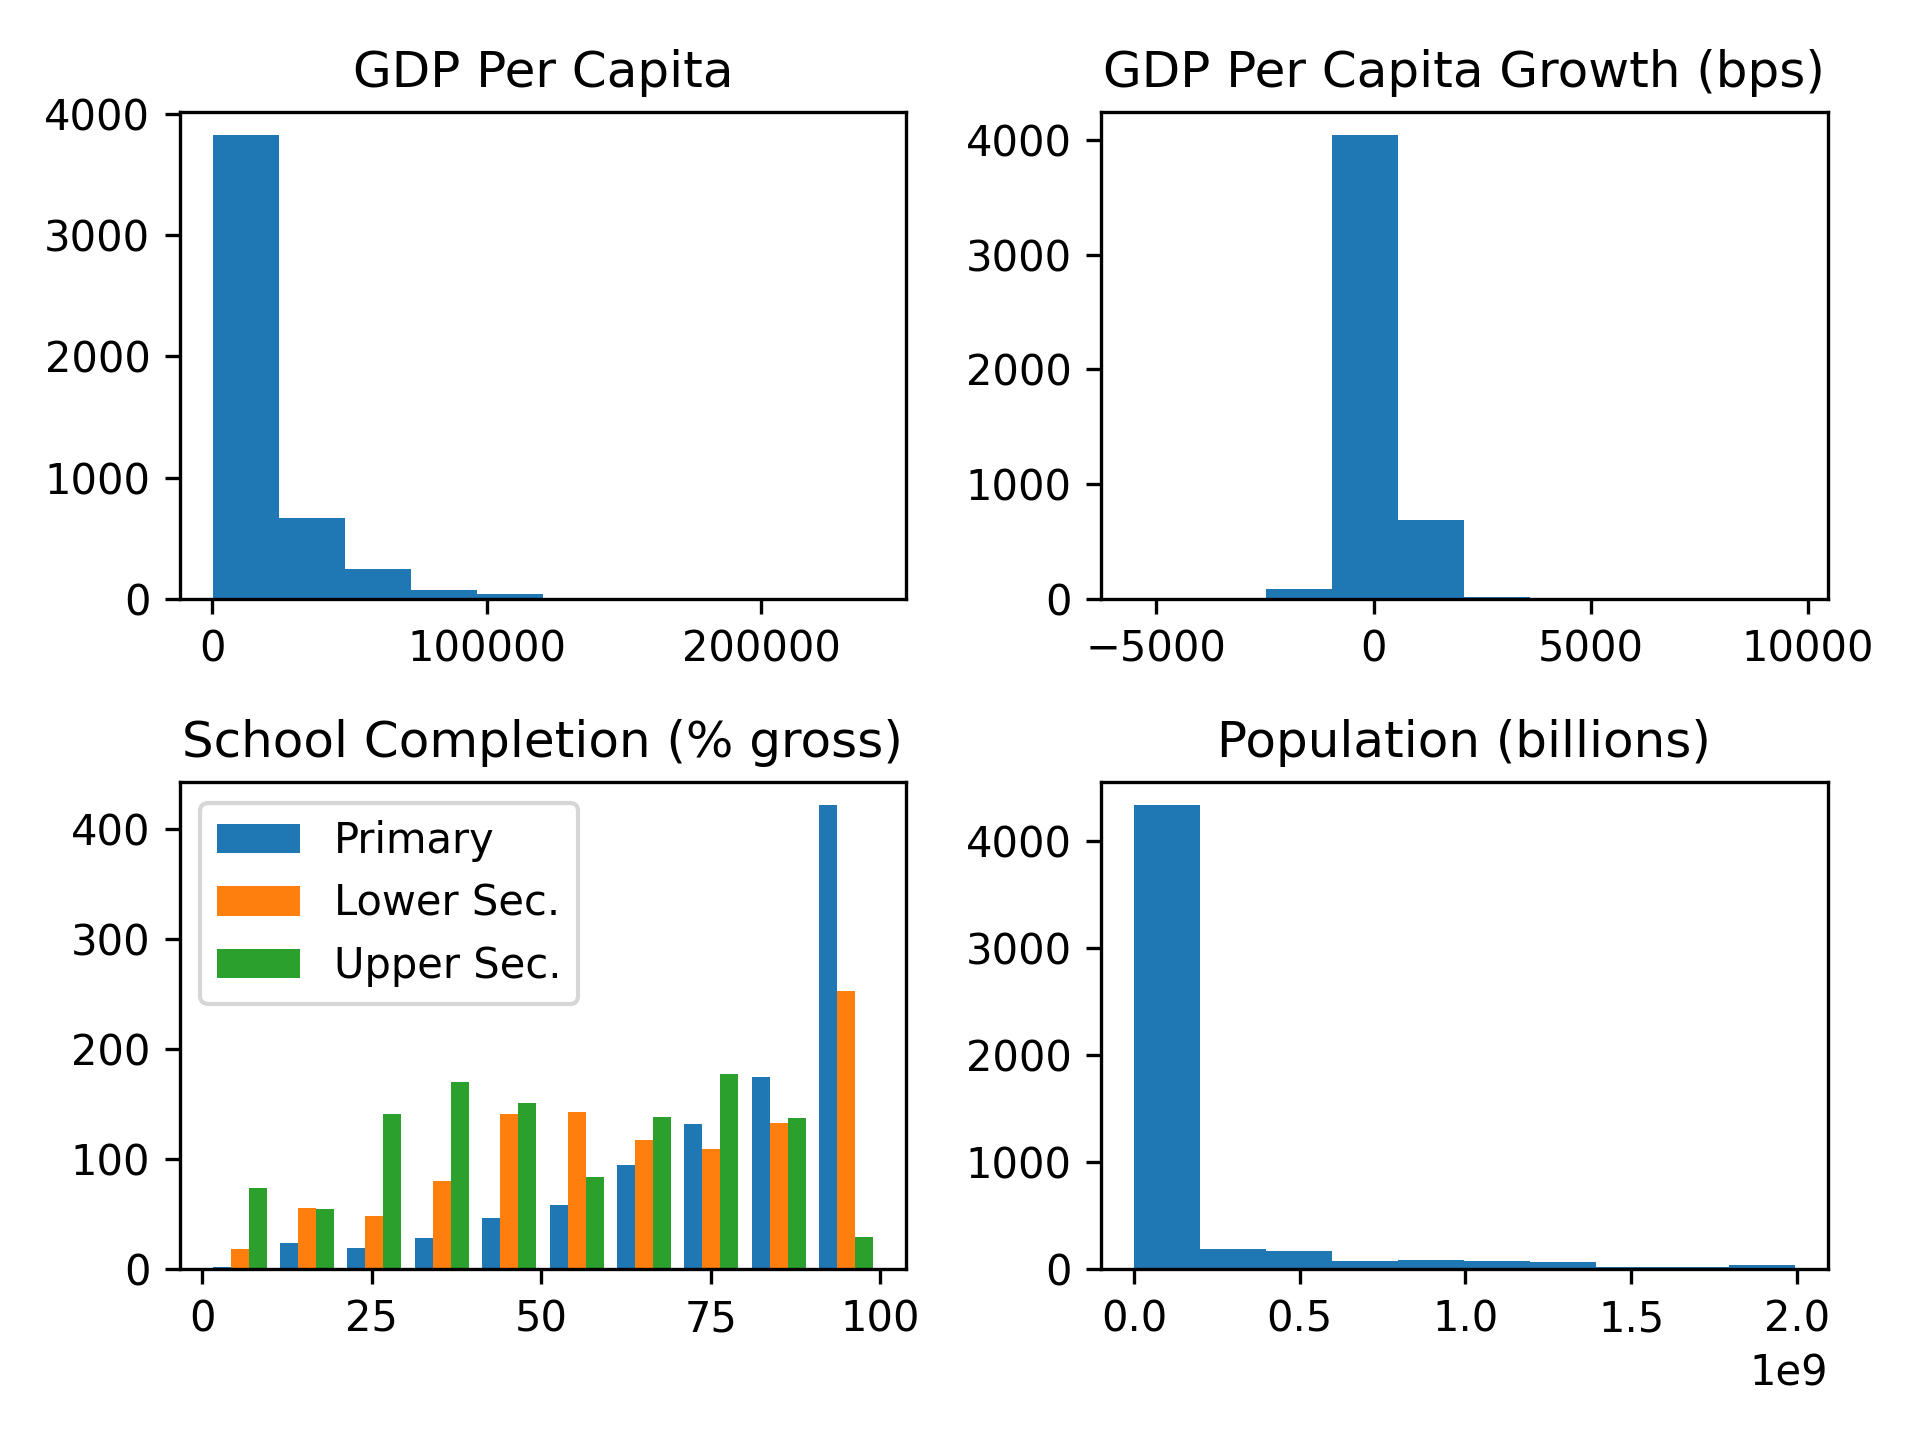
\includegraphics[width=\textwidth]{../charts/wdi.png}
% \end{frame}

\begin{frame}
    \frametitle{World Bank Data}
    \framesubtitle{Missing data}
    \centering
    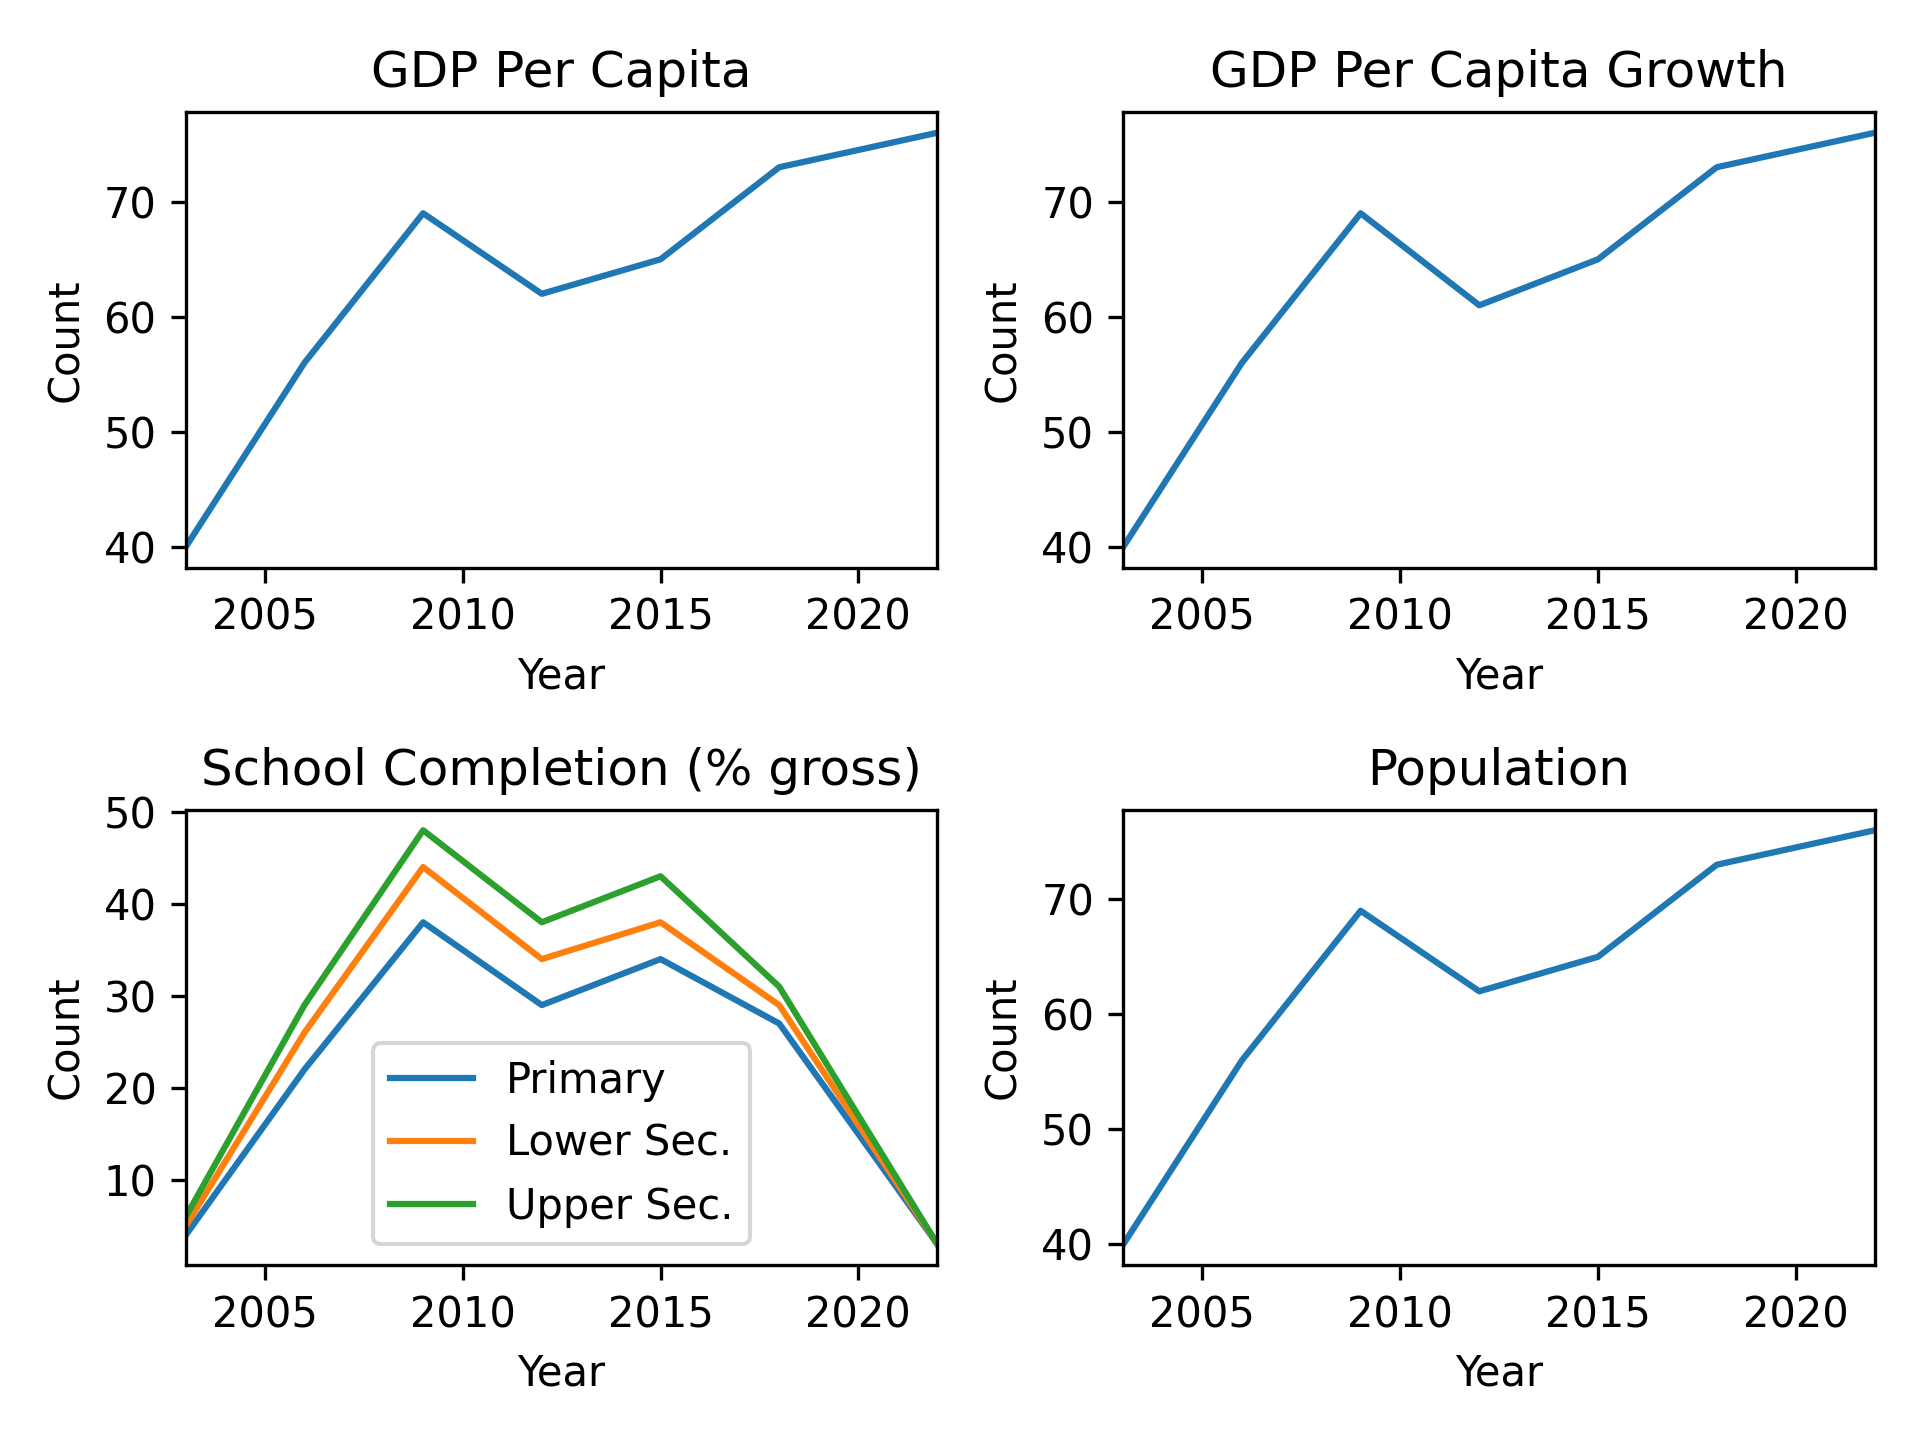
\includegraphics[width=\textwidth]{../charts/wdi-count.png}
\end{frame}

\subsection{Null Imputation}
\begin{frame}{Imputing nulls}{Using XGBoost for better predictions}
    \begin{block}{Data is not missing at random}
        School completion data is only available for a maximum of 80 countries per year and has high variance in this availablility.
        This is the most limiting factor in the analysis.
    \end{block}

    \begin{block}{Predicting missing values}
        XGBoost is a tree-based model that has built-in null handling. I use the remaining variables to predict school completion rates and EIU democracy scores.
        Achieves significantly higher accuracy than linear regression.
    \end{block}
    
\end{frame}

\subsection{IMO}
\begin{frame}{IMO Scores}{The IMO is an international mathematics contest for high school students
    }
    \begin{columns}
        \column{0.5\textwidth}
            \centering
            \begin{table}
            \caption{Top 10 countries by IMO score.}
            \resizebox{\textwidth}{!}{
            \begin{tabular}{lrrr}
                \toprule
                 & IMO Score & GDPpc & GDPpc Growth \\
                Region &  &  &  \\
                \midrule
                KOR & 10.2026 & 26060.9203 & 293.8552 \\
                CHN & 9.8296 & 6424.4972 & 786.8171 \\
                USA & 9.6196 & 54346.5078 & 125.7613 \\
                RUS & 9.0800 & 10432.8366 & 277.0704 \\
                SGP & 9.0642 & 51652.4651 & 348.0543 \\
                BGR & 8.8821 & 7556.3933 & 417.7564 \\
                ROU & 8.7367 & 9432.6698 & 439.7522 \\
                HUN & 8.7153 & 13979.7009 & 262.9650 \\
                VNM & 8.5029 & 2159.2583 & 527.6404 \\
                UKR & 8.3941 & 3079.8378 & 131.9303 \\
                \bottomrule
            \end{tabular}}
        \end{table}
        \column{0.5\textwidth}
            \begin{itemize}
                \item Scores collected from 2003 to 2022
                \item Scores are transformed by $t(s) = \frac{s}{\log P}$ where $s$ is the country's raw score and $P$ is population.
                \begin{itemize}
                    \item Team size of 6 means that larger countries have an advantage due to ``genius odds''
                    \item Score is capped, so dividing by $\log P$ will correct for theoretical ceiling of performance
                \end{itemize}
            \end{itemize}
        \end{columns}
\end{frame}

\subsection{ARWU Rankings}
\begin{frame}{ARWU Rankings}{Description and Usage}
    ARWU (Academic Ranking of World Universities) is a set of university rankings based primarily on research output.
    \begin{itemize}
        \item Rankings are produced annually and are available from 2003
        \item From 2003 to 2016, 500 top universities were ranked; after 2017, 1000 were ranked.
    \end{itemize}
    
    \begin{block}{Per-Capita Scaling}
        Larger countries naturally have an advantage, so a more fair metric is
        \[ARWU_{i,t} = \frac{arwuCount_{i,t}}{P_{i,t}} \cdot 10^6 \]
        Instead, looking at ARWU insitutions per million population indicates the relative quantity of elite insitutions in a country/region.
    \end{block}
    
\end{frame}

\begin{frame}{PISA Math Scores}
    World-wide study to evaluate 15-year-old students' performance on math, science, and reading. Testing is done usually every 3 years, starting from 2000. 2021 study was delayed to 2022 due to COVID.

    \begin{itemize}
        \item This paper uses PISA mathematics data from 2003 to 2022
        \item Countries included are mostly OECD (wealthier), with some other regions/countries participating
        \item Must use weighted means because of survey methodology $math_{c, t} = \frac{\sum_{i \in c \cap t} stu\_math_i \cdot stu\_wgt_i}{\sum_{i \in c \cap t} stu\_wgt_i}$
    \end{itemize}

    As an indicator of ``elite'' academic performance, also compute the share of students in a region/country in global 1\% of test takers (benchmark score $B_{t}$):
    \[math99_{c, t} = \frac{\sum_{i \in c \cap t} (stu\_math_i \geq B_t) \cdot stu\_wgt_i}{\sum_{i \in c \cap t} stu\_wgt_i}\]
\end{frame}

\subsection{EIU Democracy Index}
\begin{frame}{EIU Democracy Index}
    \begin{columns}
        \column{0.4\textwidth}
        Index measuring the quality of democracy around the world published by the Economist Intelligence Unit.
        \begin{itemize}
            \item Published from 2006 every 2 years until 2010, annually afterwards (use XGBoost to impute missing)
            \item 0-10 scale, where 10 is democracy and 0 is autocracy.
        \end{itemize}

        \column{0.6\textwidth}
        \centering
        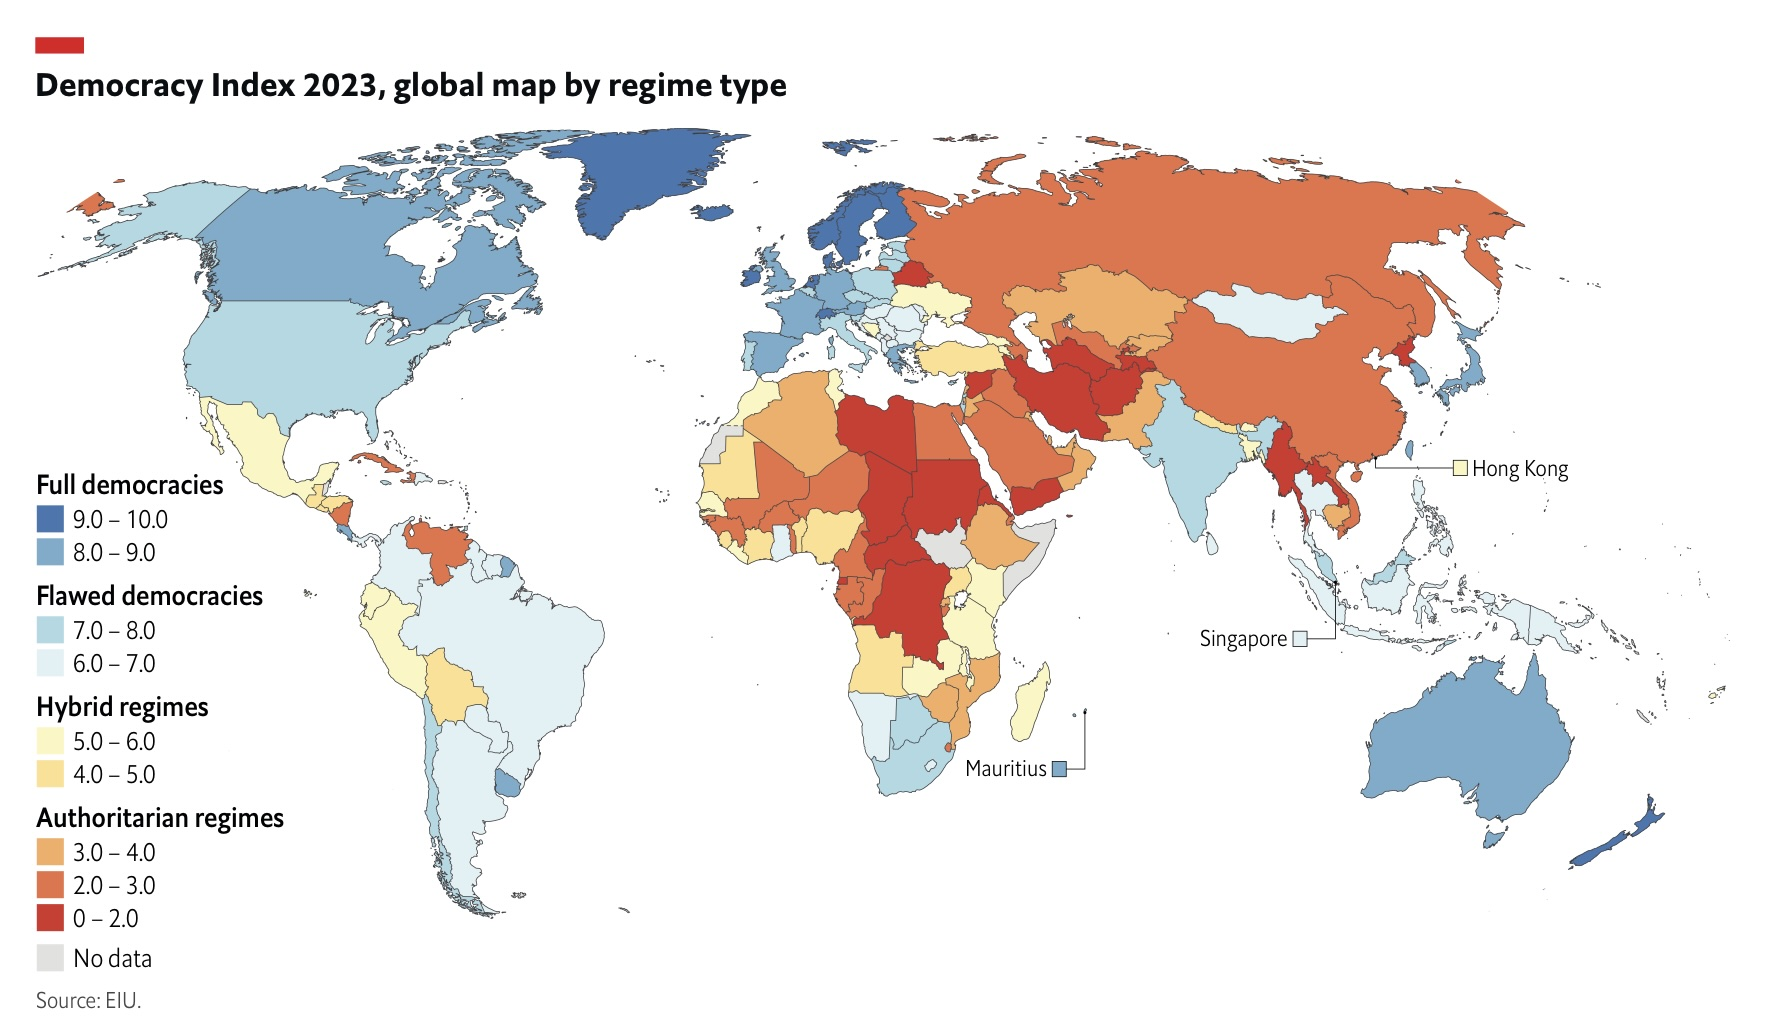
\includegraphics[width=\textwidth]{../charts/eiu_2023.jpg}
    \end{columns}
    
\end{frame}
\subsection{Summary}

\begin{frame}{Rationale for variables}{What is defined as ``elite''?}
    \begin{block}{IMO Scores}
        Indicator for a country's (and region's) ability to develop and identify pinncale STEM talent at high school level. Requires students to take it seriously.
    \end{block}

    \begin{block}{ARWU Rankings}
        Indicator for a country's (and region's) ability to produce exellence in research output.
    \end{block}

    \begin{block}{\% in PISA 99th percentile}
        Average scores are controlled for, so this indicates degree of right skew and wider academic culture.
    \end{block}
\end{frame}

\section{Empirical Results}
\begin{frame}{Model specification}
    \small
    Let elite indicators be: $math99, ARWU, IMO$.
    For the sake of concision, let $E_{i,t}$ be a 1 by 4 matrix defined as:
    \[E_{i,t} = 
    \begin{bmatrix}
        math99_{i, t} & ARWU_{i, t} & IMO_{i, t}
    \end{bmatrix}
    \] for country/region $i$ in year $t$.
    For control variables, $I_{i, t}$ is the matrix of variables and $\alpha$ is coefficients.
    \begin{equation}
        Y_{i, t} = \beta_0 + \lambda E_{i, t} + \alpha I_{i, t} + T_t + C_i + \epsilon_{i, t}
    \end{equation}
    where $T,C$ represent time and entity dummies respectively and $Y_{i,t}$ be the GDP per capita growth in basis points for a country/region $i$ and year $t$.
    \textbf{Controls: school completion rates, GDP per capita, PISA average math score, democracy index, population}
\end{frame}

\begin{frame}{Relationships}
    \centering
    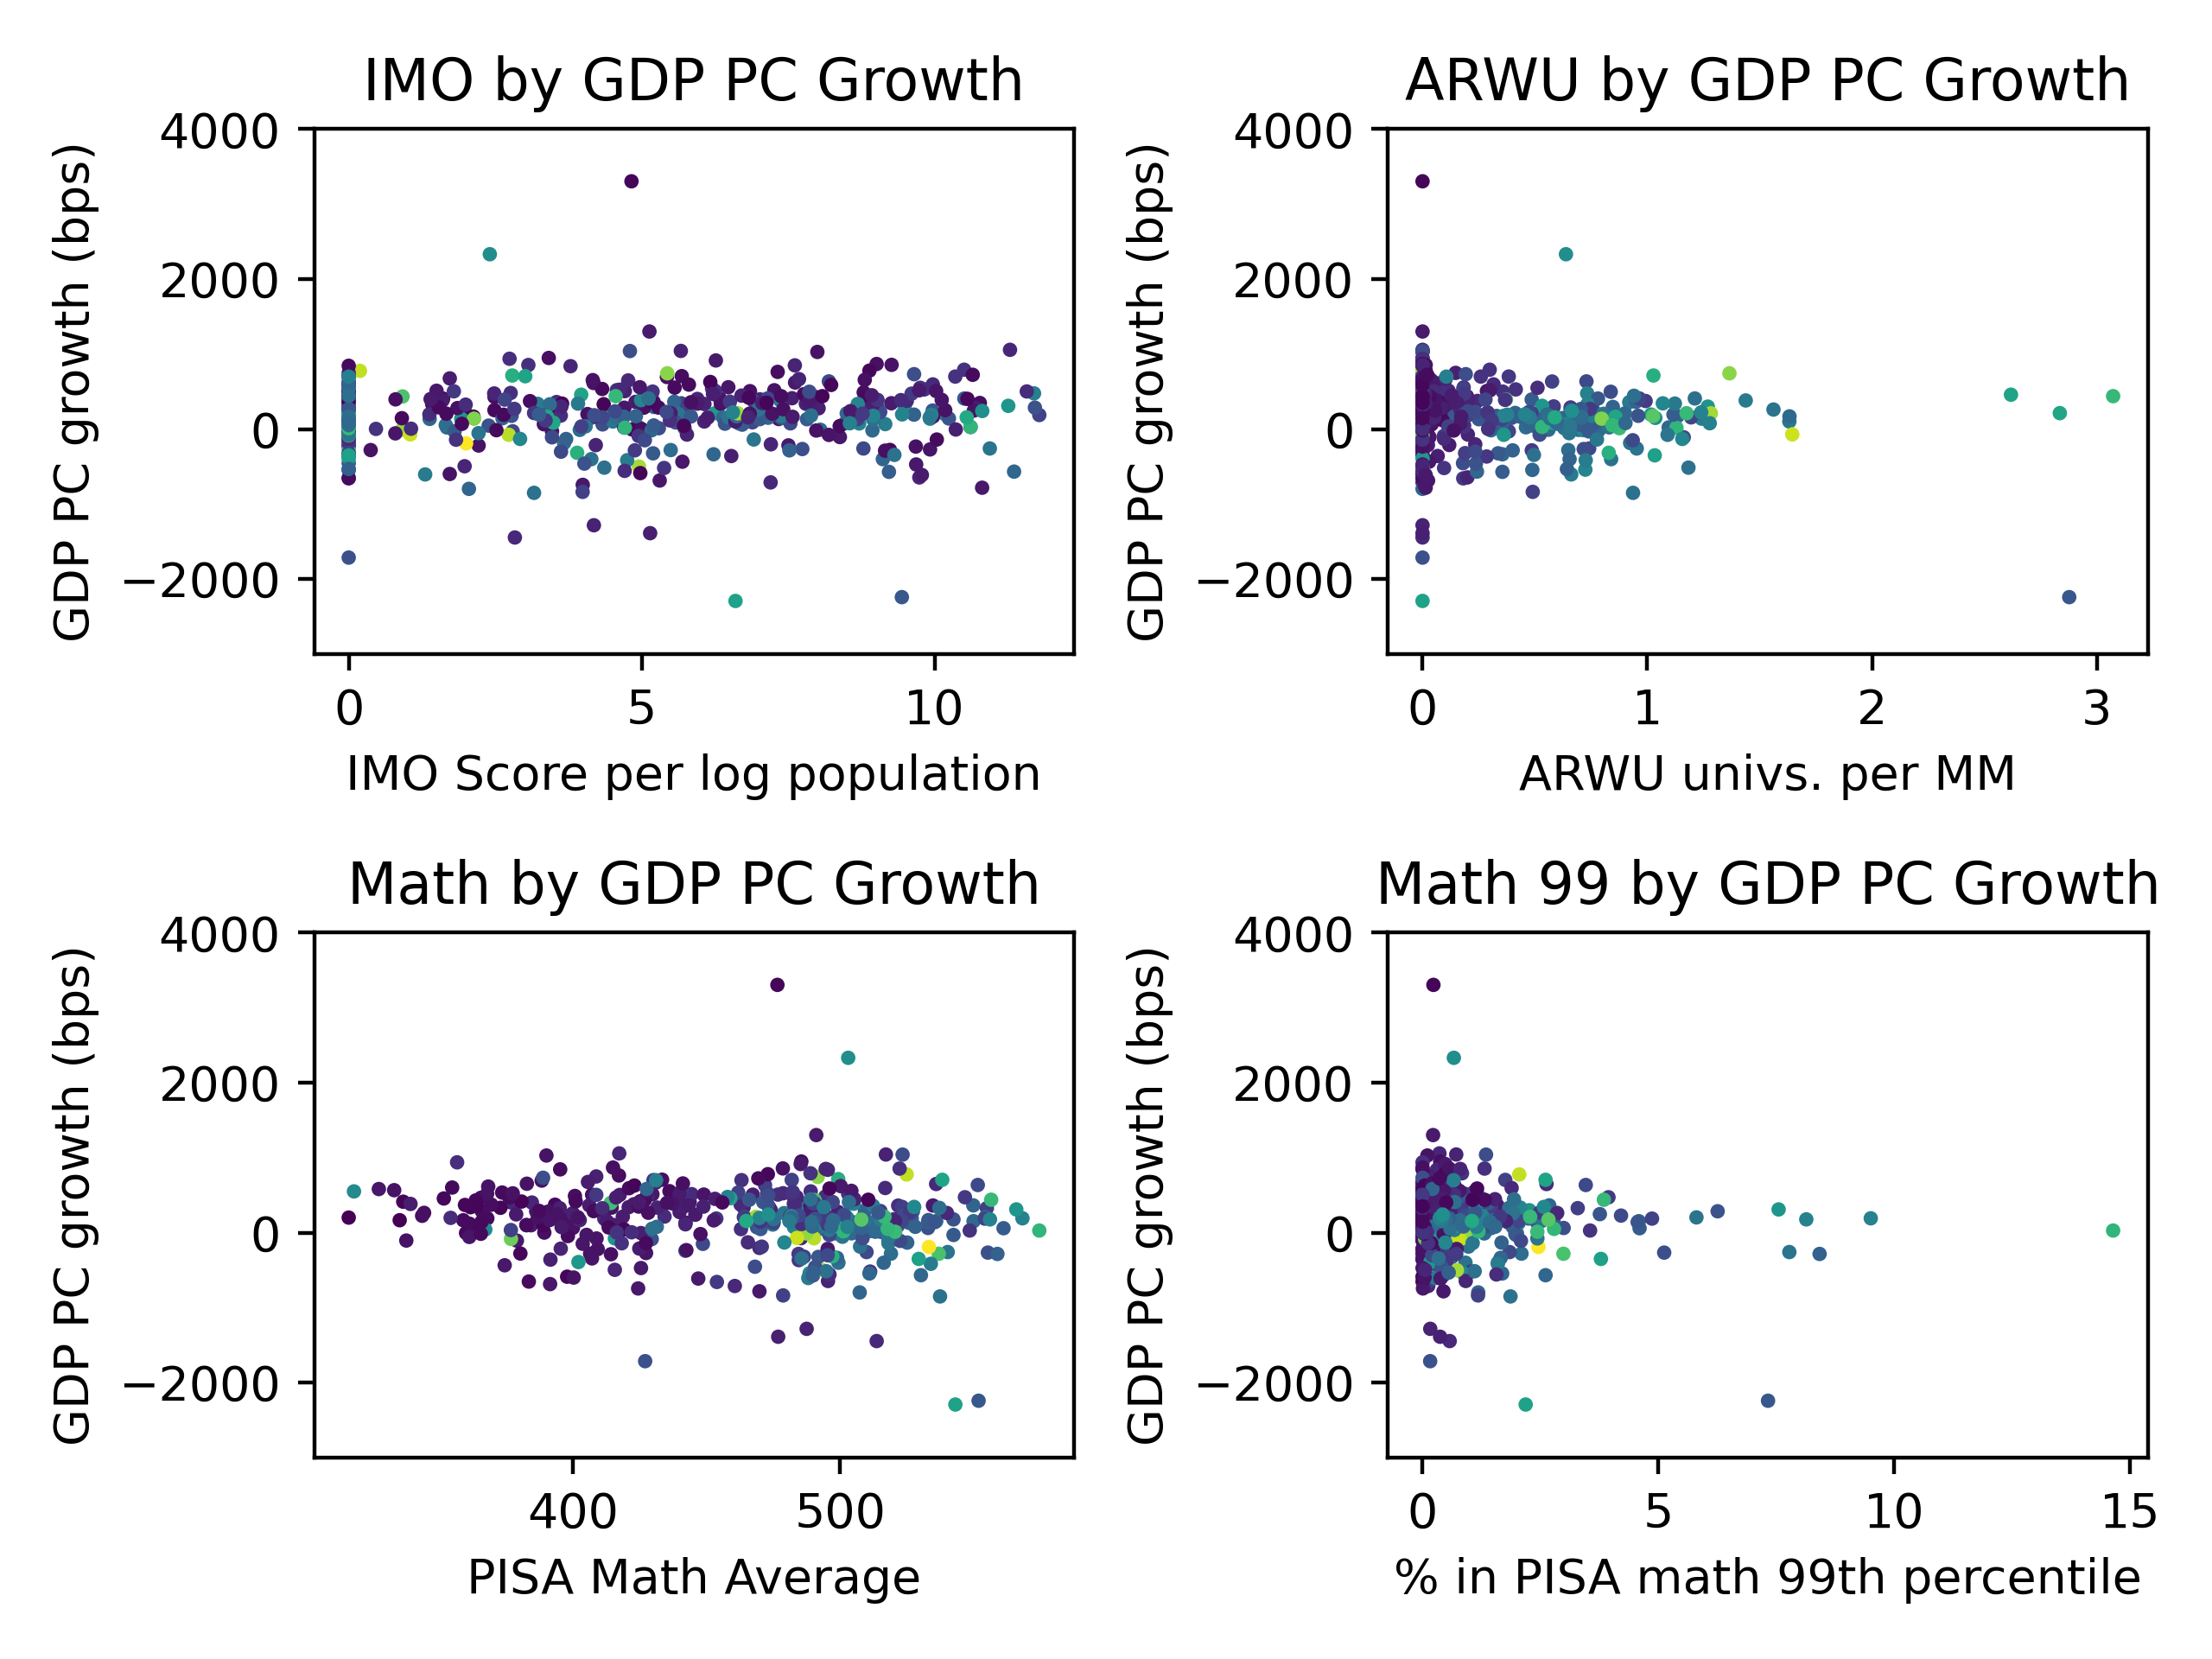
\includegraphics[width=\textwidth]{../charts/relationships.png}
\end{frame}
\subsection{Regression tables}
\begin{frame}{PISA panel regression}{Highly dependent on model specification due to rich country bias and limited variation}
    \begin{table}[!htbp] \centering
        \resizebox{\linewidth}{!} {
            \begin{tabular}{@{\extracolsep{5pt}}lcccc}
                \\[-1.8ex]\hline
                \hline \\[-1.8ex]
                & \multicolumn{4}{c}{\textit{Dependent variable: GDP Per Capita Growth (bps)}} \
                \cr \cline{2-5}
                \\[-1.8ex] & \multicolumn{1}{c}{Model 1 (base)} & \multicolumn{1}{c}{Model 2} & \multicolumn{1}{c}{Model 3 (Time FE)} & \multicolumn{1}{c}{Model 4 (Time + Entity FE)}  \\
                \hline \\[-1.8ex]
                 PISA Math in global P99 & -31.228$^{*}$ & -38.928$^{*}$ & -34.569$^{*}$ & -115.492$^{***}$ \\
                & (16.314) & (20.802) & (17.850) & (36.599) \\
                 IMO score per log population & 10.674$^{*}$ & 4.924$^{}$ & 3.122$^{}$ & -11.158$^{}$ \\
                & (6.363) & (7.470) & (6.441) & (15.728) \\
                 ARWU insitutions & -166.641$^{**}$ & -162.705$^{*}$ & -176.049$^{**}$ & -159.960$^{}$ \\
                & (68.800) & (86.871) & (72.281) & (112.884) \\
                 Time Effects & No & No & Yes & Yes \\
                 Fixed Effects & No & No & No & Yes \\
                 Controls & No & Yes & Yes & Yes \\
                 Entities & 89 & 89 & 89 & 89 \\
                \hline \\[-1.8ex]
                 Observations & 440 & 440 & 440 & 440 \\
                 $R^2$ & 0.037 & 0.077 & 0.374 & 0.553 \\
                 Adjusted $R^2$ & 0.031 & 0.056 & 0.351 & 0.414 \\
                 Residual Std. Error & 445.700 (df=436) & 439.888 (df=429) & 364.790 (df=423) & 346.511 (df=335) \\
                 F Statistic & 5.616$^{***}$ (df=3; 436) & 3.589$^{***}$ (df=10; 429) & 15.813$^{***}$ (df=16; 423) & 3.983$^{***}$ (df=104; 335) \\
                \hline
                \hline \\[-1.8ex]
                \textit{Note:} & \multicolumn{4}{r}{$^{*}$p$<$0.1; $^{**}$p$<$0.05; $^{***}$p$<$0.01} \\
                \end{tabular}
        }
        \end{table}
        \small
        \begin{itemize}
            \item Introducing controls and time effects do not have a major effect on coefficients; elite indicators are not highly correlated with controls
            \item Country/region fixed effects have small effect on ARWU variable, large effects on PISA math 99 and IMO variables
        \end{itemize}
\end{frame}

\begin{frame}{PISA yearly regression}
    \begin{table}[!htbp] \centering
        \resizebox{\linewidth}{!} {
            \begin{tabular}{@{\extracolsep{1pt}}lcccccccc}
                \\[-1.8ex]\hline
                \hline \\[-1.8ex]
                & \multicolumn{8}{c}{\textit{Dependent variable: GDP Per Capita Growth (bps)}} \
                \cr \cline{2-9}
                \\[-1.8ex] & \multicolumn{1}{c}{2003} & \multicolumn{1}{c}{2006} & \multicolumn{1}{c}{2009} & \multicolumn{1}{c}{2012} & \multicolumn{1}{c}{2015} & \multicolumn{1}{c}{2018} & \multicolumn{1}{c}{2022} & \multicolumn{1}{c}{Panel FE}  \\
                \hline \\[-1.8ex]
                 PISA Math in global P99 & -52.490$^{}$ & -193.475$^{**}$ & 154.062$^{**}$ & 16.575$^{}$ & -34.309$^{}$ & 3.769$^{}$ & -69.681$^{**}$ & -115.492$^{***}$ \\
                & (48.524) & (84.559) & (62.680) & (36.365) & (76.140) & (27.106) & (27.702) & (36.599) \\
                 IMO score per log population & 4.478$^{}$ & -9.112$^{}$ & 14.038$^{}$ & 7.368$^{}$ & -16.622$^{}$ & 2.193$^{}$ & -0.174$^{}$ & -11.158$^{}$ \\
                & (17.327) & (20.741) & (17.012) & (13.983) & (27.567) & (7.722) & (13.474) & (15.728) \\
                 ARWU insitutions & -300.038$^{**}$ & -454.401$^{***}$ & 136.623$^{}$ & -344.990$^{**}$ & 289.270$^{}$ & 61.220$^{}$ & -829.105$^{***}$ & -159.960$^{}$ \\
                & (111.479) & (167.497) & (188.401) & (133.886) & (270.034) & (125.503) & (206.280) & (112.884) \\
                Controls & Yes & Yes & Yes & Yes & Yes & Yes & Yes & Yes \\
                \hline \\[-1.8ex]
                 Observations & 40 & 56 & 69 & 61 & 65 & 73 & 76 & 440 \\
                 $R^2$ & 0.675 & 0.499 & 0.264 & 0.302 & 0.100 & 0.294 & 0.417 & 0.553 \\
                 Adjusted $R^2$ & 0.562 & 0.387 & 0.137 & 0.162 & -0.067 & 0.180 & 0.327 & 0.414 \\
                 Residual Std. Error & 179.479 (df=29) & 365.156 (df=45) & 402.134 (df=58) & 254.369 (df=50) & 490.971 (df=54) & 180.728 (df=62) & 335.236 (df=65) & 346.511 (df=335) \\
                 F Statistic & 6.011$^{***}$ (df=10; 29) & 4.479$^{***}$ (df=10; 45) & 2.075$^{**}$ (df=10; 58) & 2.158$^{**}$ (df=10; 50) & 0.598$^{}$ (df=10; 54) & 2.581$^{**}$ (df=10; 62) & 4.649$^{***}$ (df=10; 65) & 3.983$^{***}$ (df=104; 335) \\
                \hline
                \hline \\[-1.8ex]
                \textit{Note:} & \multicolumn{8}{r}{$^{*}$p$<$0.1; $^{**}$p$<$0.05; $^{***}$p$<$0.01} \\
                \end{tabular}
        }
        \end{table}
        \small
        \begin{block}{Relationship changes from year to-year}
            \begin{itemize}
                \item 2009 is a significant outlier (coefficients now positive than negative, probably due to recession)
                \item Panel methods may ``average out'' the variations in relationship
                \item High variance in $R^2$ suggest that importance of controls, variables of interest may also not be constant
            \end{itemize}
        \end{block}
        
\end{frame}

% \begin{frame}
%     \frametitle{Non-PISA data regression}
%     \begin{table}[!htbp] \centering
%         \resizebox{\linewidth}{!} {
%             \begin{tabular}{@{\extracolsep{5pt}}lcccc}
%                 \\[-1.8ex]\hline
%                 \hline \\[-1.8ex]
%                 & \multicolumn{4}{c}{\textit{Dependent variable: GDPpcGrowth}} \
%                 \cr \cline{2-5}
%                 \\[-1.8ex] & \multicolumn{1}{c}{Model 3 (PISA)} & \multicolumn{1}{c}{Model 5 (PISA years)} & \multicolumn{1}{c}{Model 6 (All years)} & \multicolumn{1}{c}{Model 7 (All years, FE)}  \\
%                 \hline \\[-1.8ex]
%                  IMO score per log population & 10.055$^{}$ & 18.160$^{***}$ & 13.297$^{***}$ & 10.006$^{}$ \\
%                 & (8.154) & (6.517) & (3.993) & (10.776) \\
%                  ARWU insitutions & -575.550$^{***}$ & -446.996$^{**}$ & -353.730$^{***}$ & 523.241$^{*}$ \\
%                 & (213.365) & (221.189) & (131.179) & (292.381) \\
%                  ARWU insitutions x GDP PC & 0.008$^{*}$ & 0.008$^{*}$ & 0.005$^{*}$ & -0.012$^{**}$ \\
%                 & (0.004) & (0.004) & (0.002) & (0.006) \\
%                  GDP per capita & -0.004$^{**}$ & -0.005$^{***}$ & -0.004$^{***}$ & 0.002$^{}$ \\
%                 & (0.002) & (0.002) & (0.001) & (0.004) \\
%                  Primary School Completion Rate & -0.112$^{}$ & -3.530$^{**}$ & -1.754$^{}$ & -1.505$^{}$ \\
%                 & (4.338) & (1.740) & (1.227) & (4.983) \\
%                  Lower Sec. Completion Rate & 1.568$^{}$ & 5.370$^{**}$ & 1.911$^{}$ & -0.147$^{}$ \\
%                 & (3.290) & (2.445) & (1.692) & (5.035) \\
%                  Upper Sec. Completion Rate & 1.542$^{}$ & -2.365$^{}$ & 0.081$^{}$ & 1.981$^{}$ \\
%                 & (2.543) & (1.946) & (1.325) & (3.776) \\
%                  Democracy Rating & 4.167$^{}$ & 13.397$^{}$ & 19.784$^{***}$ & 87.626$^{**}$ \\
%                 & (21.249) & (11.913) & (7.637) & (37.349) \\
%                  Population & -0.000$^{*}$ & -0.000$^{}$ & -0.000$^{}$ & 0.000$^{}$ \\
%                 & (0.000) & (0.000) & (0.000) & (0.000) \\
%                  Time Effects & Yes & Yes & Yes & Yes \\
%                  Fixed Effects & No & No & No & Yes \\
%                  Entities & 48 & 103 & 137 & 137 \\
%                 \hline \\[-1.8ex]
%                  Observations & 109 & 222 & 746 & 746 \\
%                  $R^2$ & 0.402 & 0.202 & 0.380 & 0.611 \\
%                  Adjusted $R^2$ & 0.313 & 0.156 & 0.360 & 0.505 \\
%                  Residual Std. Error & 199.076 (df=94) & 240.456 (df=209) & 288.864 (df=722) & 253.976 (df=586) \\
%                  F Statistic & 4.512$^{***}$ (df=14; 94) & 4.417$^{***}$ (df=12; 209) & 19.219$^{***}$ (df=23; 722) & 5.785$^{***}$ (df=159; 586) \\
%                 \hline
%                 \hline \\[-1.8ex]
%                 \textit{Note:} & \multicolumn{4}{r}{$^{*}$p$<$0.1; $^{**}$p$<$0.05; $^{***}$p$<$0.01} \\
%             \end{tabular}
%         }
%         \end{table}
% \end{frame}

\subsection{Preliminary Interpretation}

\begin{frame}{Interpretation}
    \begin{block}{IMO Scores}
        \begin{itemize}
            \item Mostly indicates positive main relationship with GDP per capita growth (large standard errors)
            \item Negative relationship when fixed effects are included, volatile between years
        \end{itemize}
    \end{block}

    \begin{block}{PISA math 99 percentile share}
        \begin{itemize}
            \item Generally negative relationship with GDP per capita growth
            \item Negative relationship when fixed effects are included, volatile between years
        \end{itemize}
    \end{block}

    \begin{block}{ARWU insitutions per million}
        \begin{itemize}
            \item Consistent negative relationship found in regression
            \item To some degree volatile between years, but is most consistent
        \end{itemize}
    \end{block}
    
\end{frame}

\begin{frame}{Limitations}
    Regression results do not present a clear picture of the existence of a statistical relationship between elite indicators and economic growth.
    \begin{block}{Little variation in data}
        \begin{itemize}
            \item Countries and regions with PISA test scores tend to be wealthier, more developed economies
            \item Low variance within countries over time and between countries as a result
        \end{itemize}
    \end{block}

    \begin{block}{Missing data}
        \begin{itemize}
            \item XGBoost imputation is not perfect and it may have introduced bias
        \end{itemize}
    \end{block}

    \begin{block}{Reverse causality and timelines}
        \begin{itemize}
            \item Countries which grow faster may try and solidify the growth by pushing for academic exellence
            \item Lagged regression should be considered; it is not clear elite students in time $t$ have an immediate effect
        \end{itemize}
    \end{block}
    
    
\end{frame}

\begin{frame}{Limitations}{Regression framework concerns}
    \begin{block}{Unstable panel compared to yearly results}
        The panel methods mask some of the year-to-year changes in relationships.
    \end{block}

    \begin{block}{Omitted Variable Bias}
        Large changes in relationship magnitude and direction suggests that omitted variable bias is a big problem.
    \end{block}

    \begin{block}{Heterogeneity}
        No time for this today, but I have other models which include interactions to examine this. Highly possible richer/poorer countries experience different effects.
    \end{block}
    
    
\end{frame}

\section{Appendix}
\begin{frame}{Appendix: convergence and divergence in elite indicators}
    \centering
    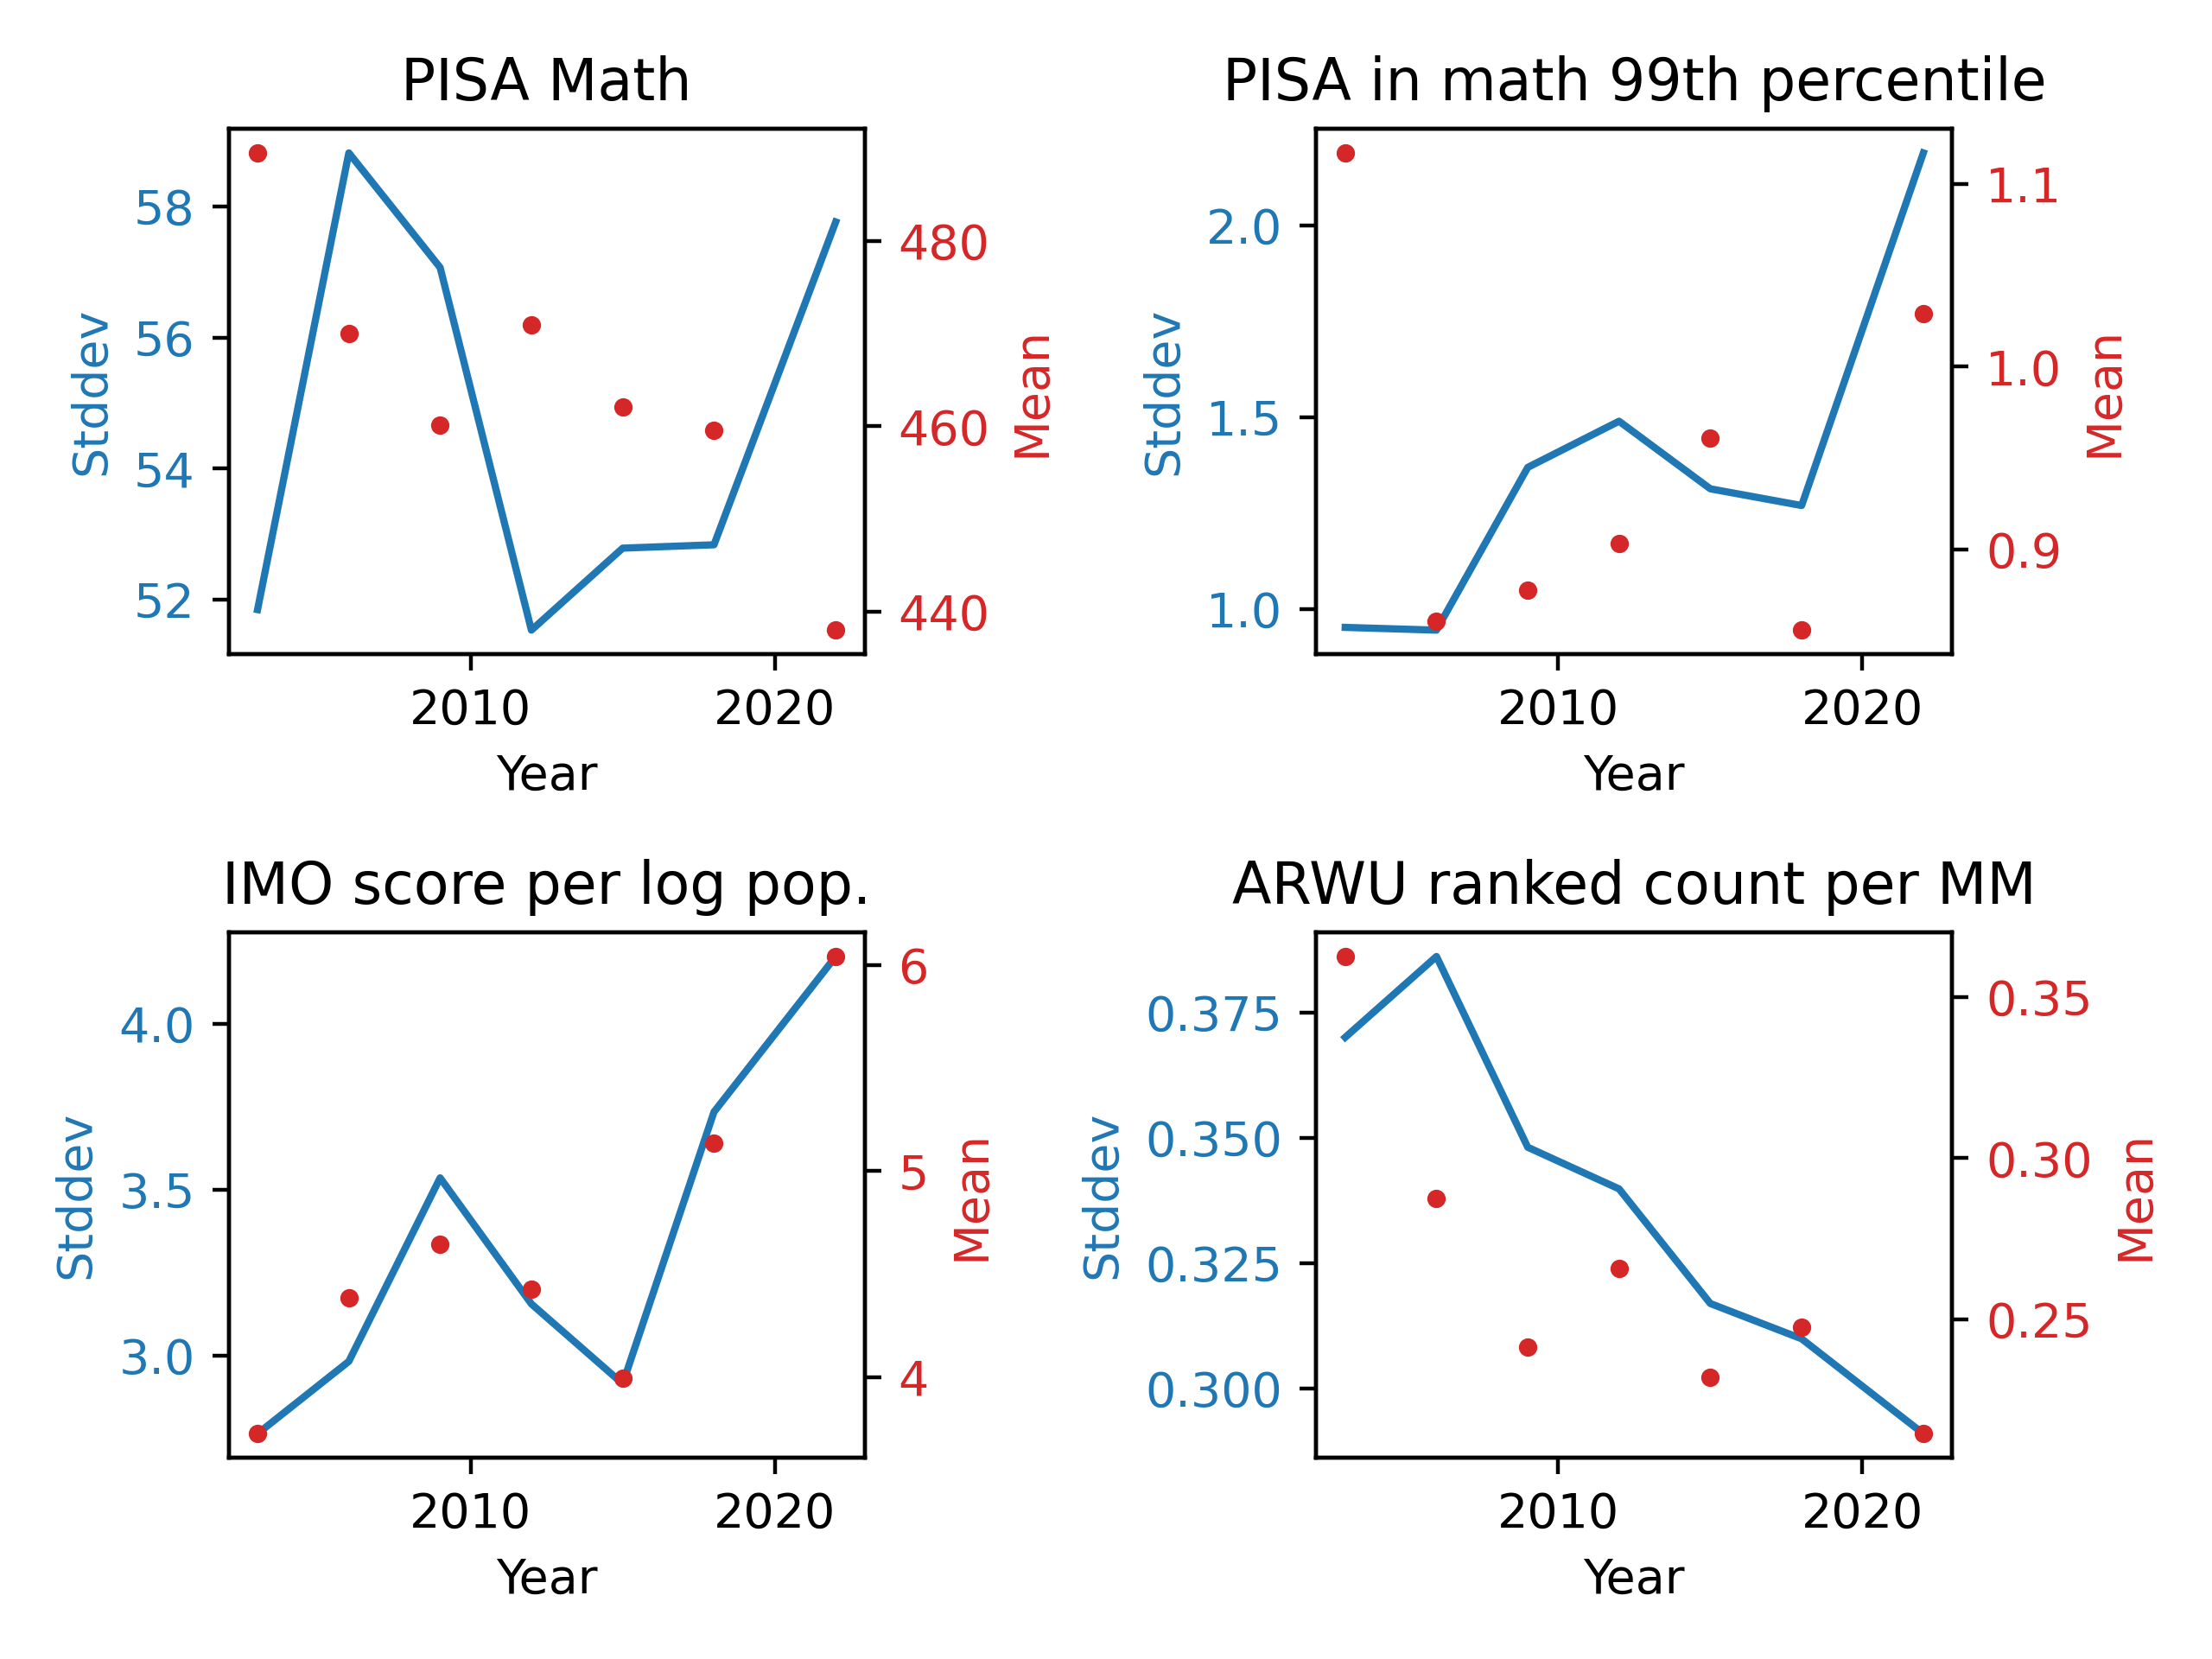
\includegraphics[width=\textwidth]{../charts/std-dev.png}
\end{frame}

\begin{frame}{Appendix: elite indicators and GDP per capita}
    \centering
    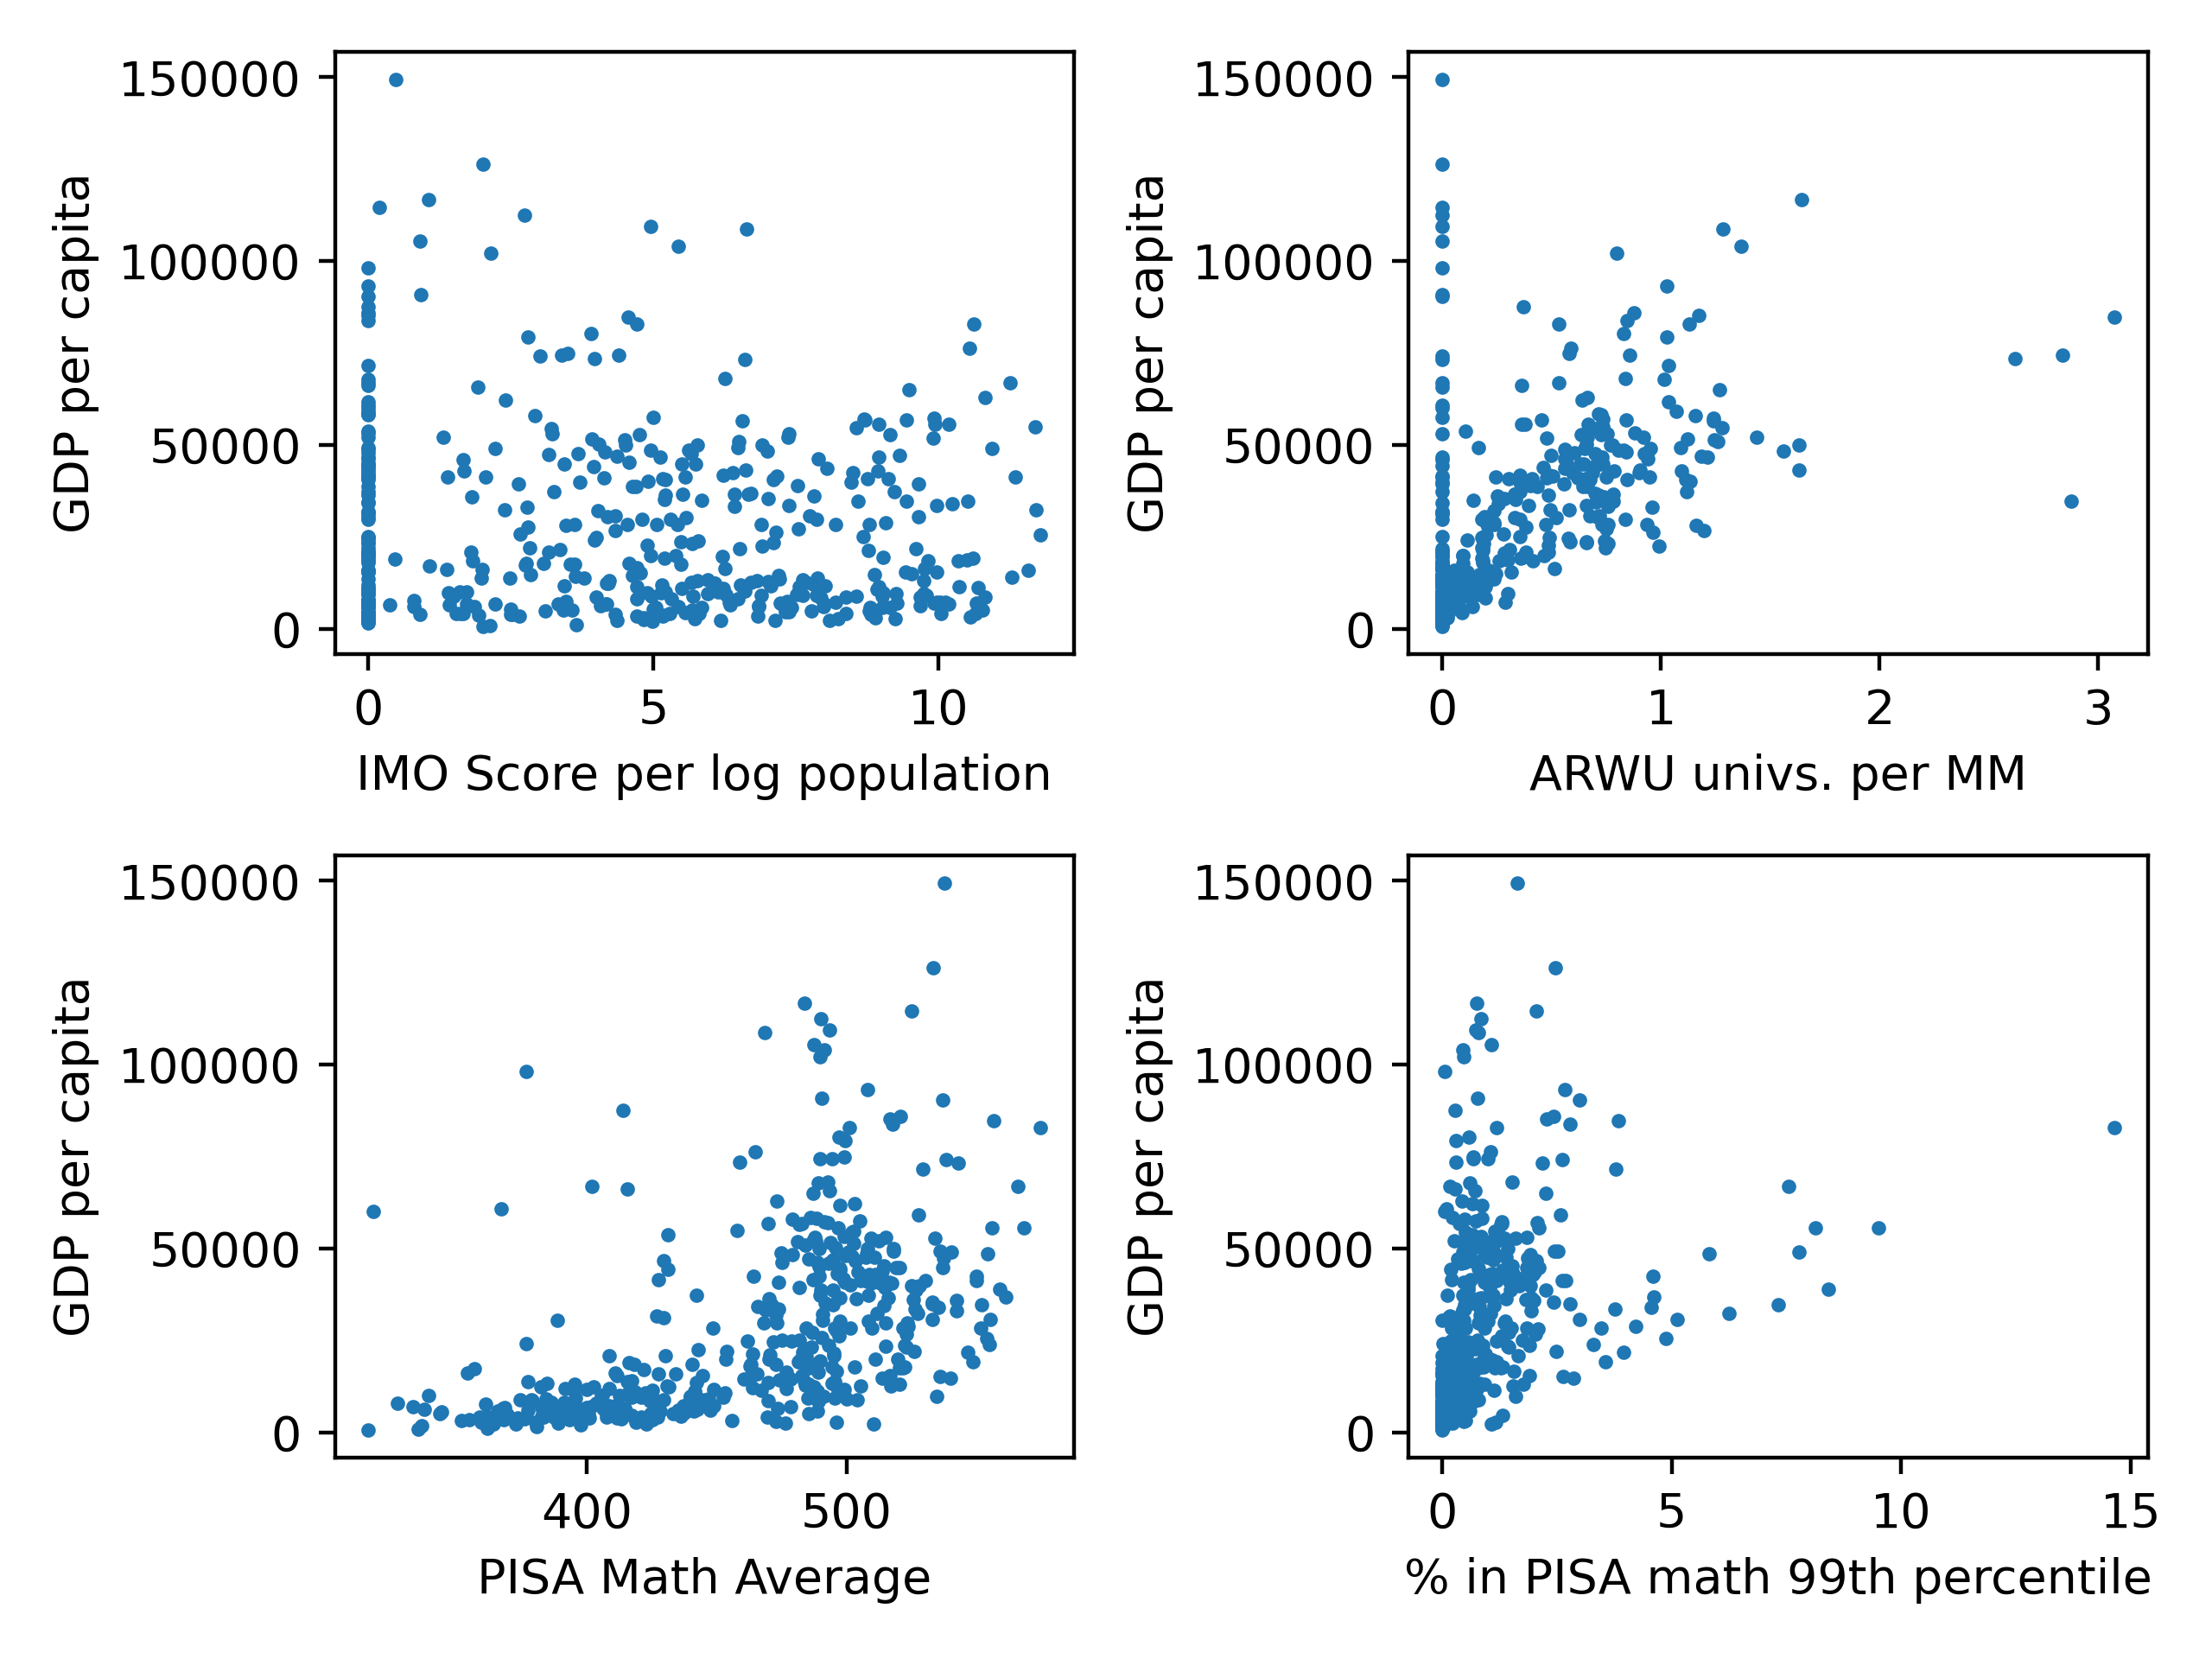
\includegraphics[width=\textwidth]{../charts/relationships-gdp-pc.png}
\end{frame}

\begin{frame}{Appendix: Summary Statistics}
    \begin{table}
        \caption{Summary Statistics}
        \resizebox{\linewidth}{!} {
            \begin{tabular}{lrrrrr}
                & Count & Mean & Std & Min & Max \\
                \\[-1.8ex]\hline
                \hline \\[-1.8ex]
               GDP per capita & 441.00 & 28463.99 & 25255.10 & 543.11 & 149461.79 \\
               GDP per capita growth (bps) & 440.00 & 169.06 & 452.68 & -2292.68 & 3303.05 \\
               EIU Democracy Index & 441.00 & 7.25 & 1.77 & 1.93 & 9.93 \\
               Primary Completion & 441.00 & 90.00 & 10.25 & 51.35 & 101.95 \\
               Lower Sec. Completion & 441.00 & 77.89 & 17.14 & 29.21 & 101.97 \\
               Upper Sec. Completion & 441.00 & 62.20 & 18.48 & 18.44 & 97.40 \\
               Population & 441.00 & 35318600.19 & 59445620.16 & 34000.00 & 333287557.00 \\
               ARWU per million pop ranked & 441.00 & 0.26 & 0.33 & 0.00 & 1.54 \\
               IMO score per log pop & 441.00 & 4.72 & 3.49 & 0.00 & 11.79 \\
               PISA math in global 1\% & 441.00 & 0.94 & 1.46 & 0.00 & 14.64 \\
               PISA math & 441.00 & 461.93 & 56.23 & 315.96 & 574.66 \\
               \end{tabular}
        }
    \end{table}
    \begin{table}
        \tiny
        \caption{Pre-imputation Statistics}
        \begin{tabular}{lrrrrr}
         & Count & Mean & Std & Min & Max \\
         \\[-1.8ex]\hline
         \hline \\[-1.8ex]
        EIU Democracy Index & 323.00 & 7.09 & 1.78 & 1.93 & 9.93 \\
        Primary Completion & 157.00 & 90.29 & 10.31 & 51.35 & 100.00 \\
        Lower Sec. Completion & 179.00 & 76.63 & 20.03 & 29.21 & 99.98 \\
        Upper Sec. Completion & 198.00 & 62.32 & 20.58 & 18.44 & 97.40 \\
        \end{tabular}
        \end{table}
\end{frame}

\begin{frame}{Appendix: Imputation results}{School completion rates}
    \centering
    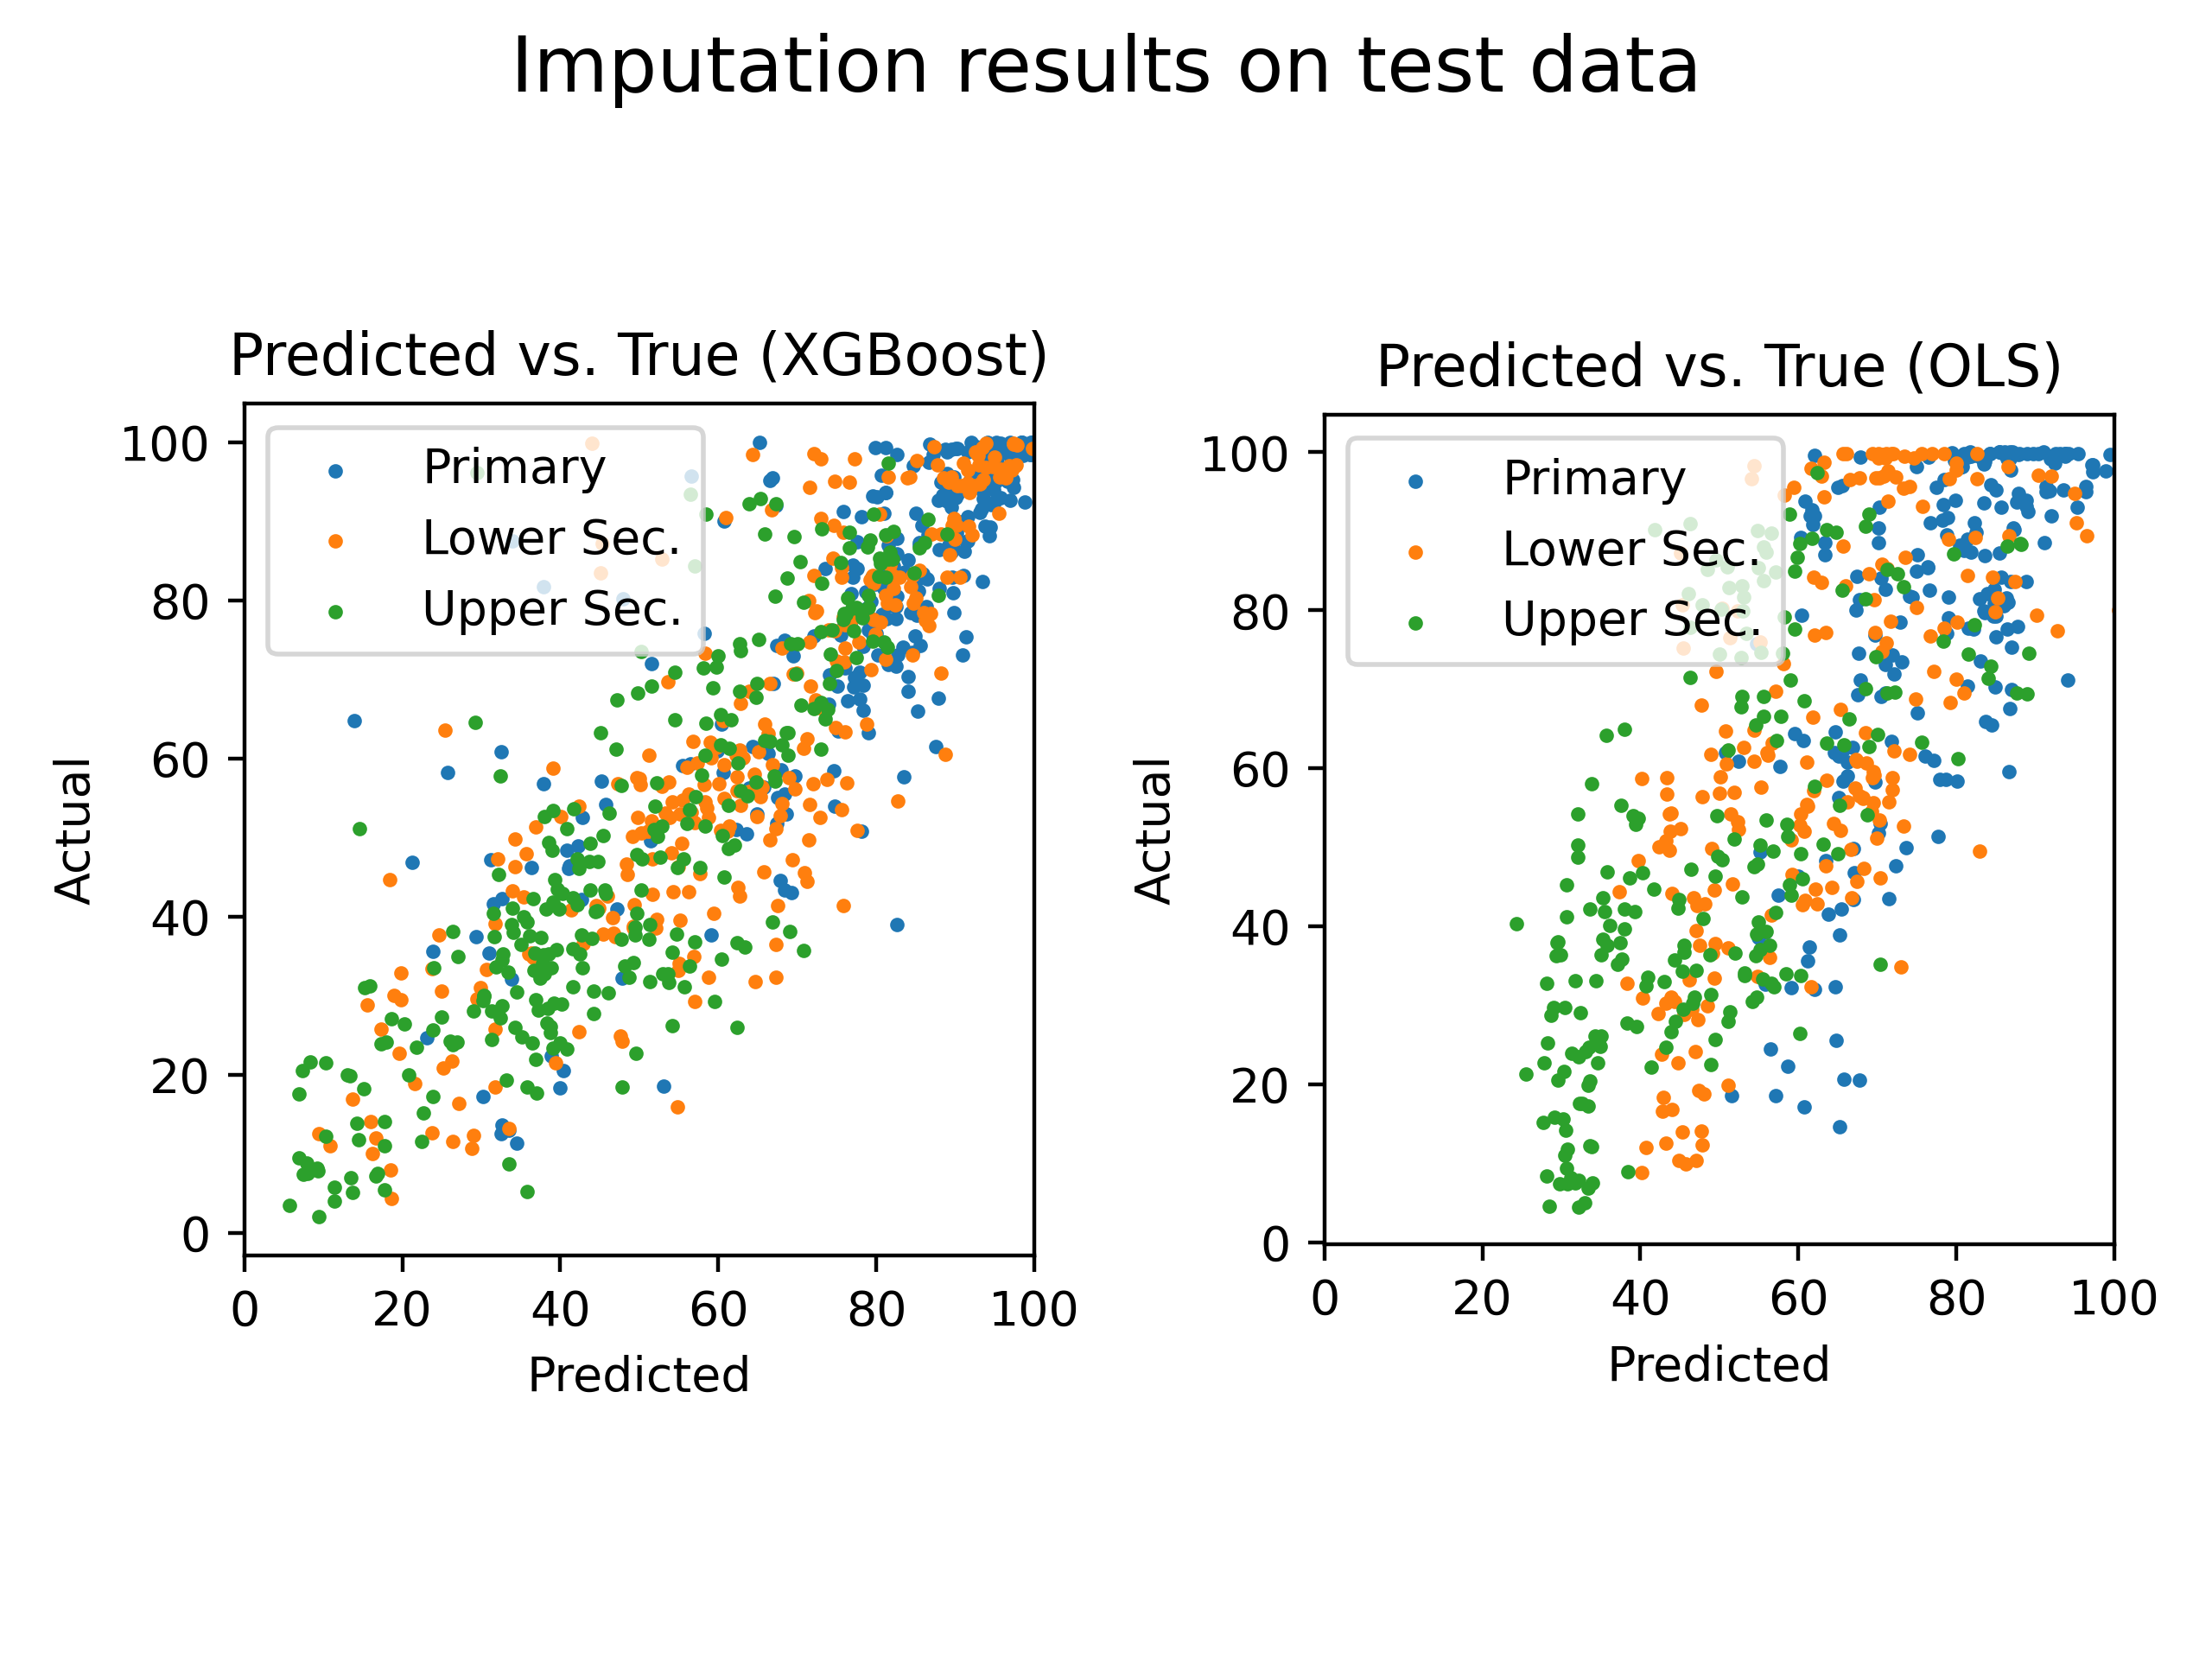
\includegraphics[width=\textwidth]{../build/xgboost.png}
\end{frame}

\begin{frame}{Appendix: Imputation results}{EIU Democracy Score}
    \centering
    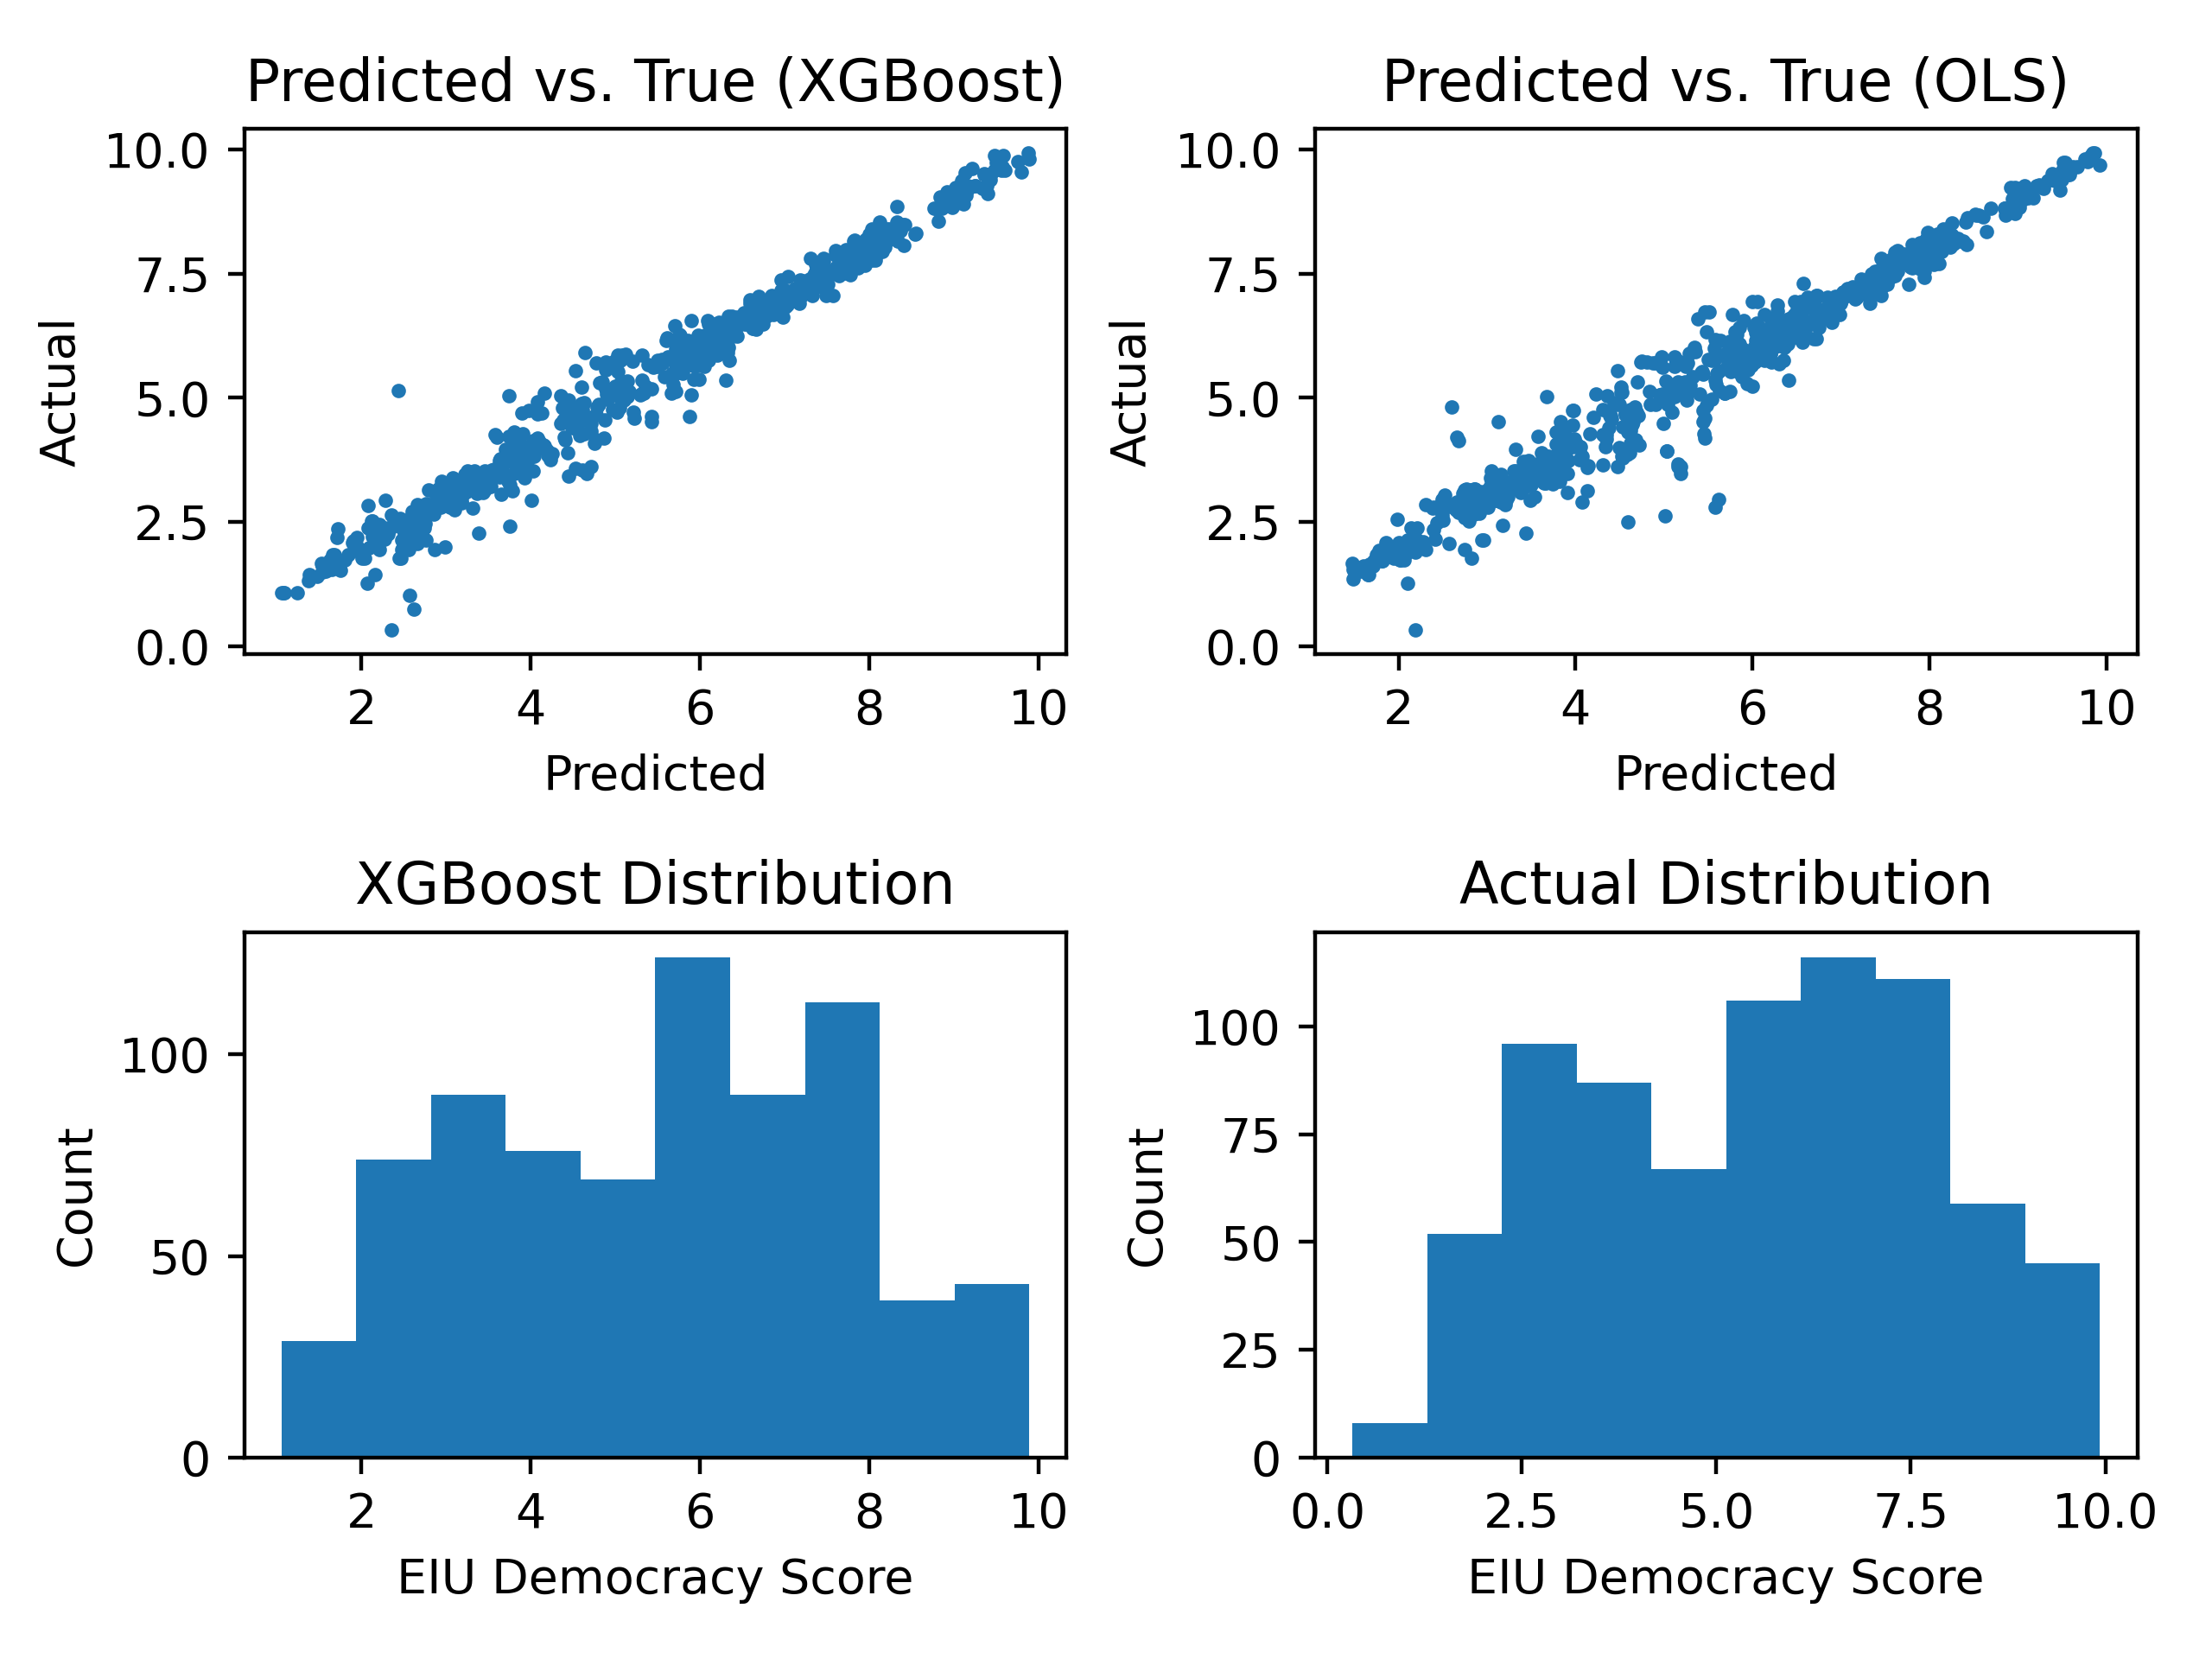
\includegraphics[width=\textwidth]{../build/eiu_xgboost.png}
\end{frame}

\begin{frame}{Appendix: PISA panel regression}{Without imputation}
    \begin{table}[!htbp] \centering
        \resizebox{\linewidth}{!} {
            \begin{tabular}{@{\extracolsep{5pt}}lcccc}
                \\[-1.8ex]\hline
                \hline \\[-1.8ex]
                & \multicolumn{4}{c}{\textit{Dependent variable: GDP Per Capita Growth (bps)}} \
                \cr \cline{2-5}
                \\[-1.8ex] & \multicolumn{1}{c}{Model 1 (base)} & \multicolumn{1}{c}{Model 2} & \multicolumn{1}{c}{Model 3 (Time FE)} & \multicolumn{1}{c}{Model 4 (Time + Entity FE)}  \\
                \hline \\[-1.8ex]
                 PISA Math in global P99 & -31.228$^{*}$ & 5.985$^{}$ & 8.659$^{}$ & 25.421$^{}$ \\
                & (16.314) & (22.468) & (21.493) & (84.291) \\
                 IMO score per log population & 10.674$^{*}$ & 6.824$^{}$ & 12.529$^{}$ & 50.506$^{}$ \\
                & (6.363) & (9.440) & (8.631) & (32.187) \\
                 ARWU insitutions & -166.641$^{**}$ & -190.750$^{}$ & -249.208$^{**}$ & -454.384$^{}$ \\
                & (68.800) & (127.229) & (116.476) & (351.559) \\
                 Time Effects & No & No & Yes & Yes \\
                 Fixed Effects & No & No & No & Yes \\
                 Controls & No & Yes & Yes & Yes \\
                \hline \\[-1.8ex]
                 Observations & 440 & 112 & 112 & 112 \\
                 $R^2$ & 0.037 & 0.204 & 0.383 & 0.715 \\
                 Adjusted $R^2$ & 0.031 & 0.125 & 0.294 & 0.355 \\
                 Residual Std. Error & 445.700 (df=436) & 236.761 (df=101) & 212.750 (df=97) & 203.207 (df=49) \\
                 F Statistic & 5.616$^{***}$ (df=3; 436) & 2.587$^{***}$ (df=10; 101) & 4.294$^{***}$ (df=14; 97) & 1.987$^{***}$ (df=62; 49) \\
                \hline
                \hline \\[-1.8ex]
                \textit{Note:} & \multicolumn{4}{r}{$^{*}$p$<$0.1; $^{**}$p$<$0.05; $^{***}$p$<$0.01} \\
                \end{tabular}
        }
        \end{table}
        \small
        \begin{itemize}
            \item Relationships are very different from imputed version
            \item Some countries are missing in this regression and some years as well
            \item School completion rates are only available for certain years and we have seen the relationship to be volatile year-to-year
        \end{itemize}
\end{frame}



\end{document}